\documentclass{article}
\usepackage{tikz}
\usepackage{tkz-euclide}
\usetikzlibrary{calc,intersections}
\usepackage{graphicx}
\usepackage{booktabs}
\usepackage{amsmath}
\newcommand{\Wheel}[3]{
  \begin{scope}[shift={#1},rotate=#2]
    \draw[rounded corners=9,#3] (-1,-5) rectangle (1,5);
  \end{scope}
}

\begin{document}

\bigskip
\begin{tikzpicture}[x=3mm,y=3mm]
  \draw (0,0) -- (10,0);
  \draw[fill,red] (-0.3,0) rectangle (0.3,20);
  \Wheel{(0,0)}{0}{black};
  \begin{scope}[shift={(0,20)},rotate=40]
    \draw[dashed] (0,-7) -- (0,7);
    \draw[dashed] (3,0) -- (-35,0);
    \Wheel{(0,0)}{0}{black};
  \end{scope}
  \coordinate (P) at (-{20/tan(40)},0);
  \draw[red] (P) circle [radius=2pt];
  \draw[dashed] (0,0) -- (P);
  % \Wheel{(0,20)}{60}{red!30!blue};
\end{tikzpicture}


\section*{Geometric Path Planning}

Using Mozzi-Chasles' theorem, any rigid body displacement can be produced by a combination of
translation along a line and a rotation about an axis parallel to that line.

Given the initial location and heading at both the starting point and target points,
we want to compute the path comprised by translation and rotation(s) as described by 
the above theorem.
Let $E$ be the intersection of the two heading lines (green and red in the diagrams).
We will analyze several major cases depending on the relative position of $E$
with respect to the two headings.


\begin{table}
  \begin{tabular}{ccccll}
    \toprule
    Overall Turn  & \multicolumn{2}{c}{Relative position of $E$ w.r.t.} & Path           & Comment                            \\
                  & start heading                                       & target heading &                                    \\
    \midrule
    $< 180^\circ$ & in front                                            & behind         & single turn                        \\
    $> 180^\circ$ & behind                                              & in front       & single turn                        \\
    any           & in front                                            & in front       & double turns & converging headings \\
    any           & behind                                              & behind         & double turns & diverging headings  \\
    \bottomrule
  \end{tabular}
\end{table}

\subsection*{Single Turn Paths}
In Figure~\ref{fig:path1turnacute}, the bike starts at point $A$ with its heading shown by
the green arrow and its target is point $C$ with its heading shown by the red arrow,
and both are pointing \textbf{in a general opposite direction}.
The extending headings are shows by the dotted lines intersected at $E$.
Line $EF$ is the angle bisector of the both heading lines, and point $F$ is the
pivot of rotation.

\begin{figure}[hbt]
  \begin{tabular}{cc}
    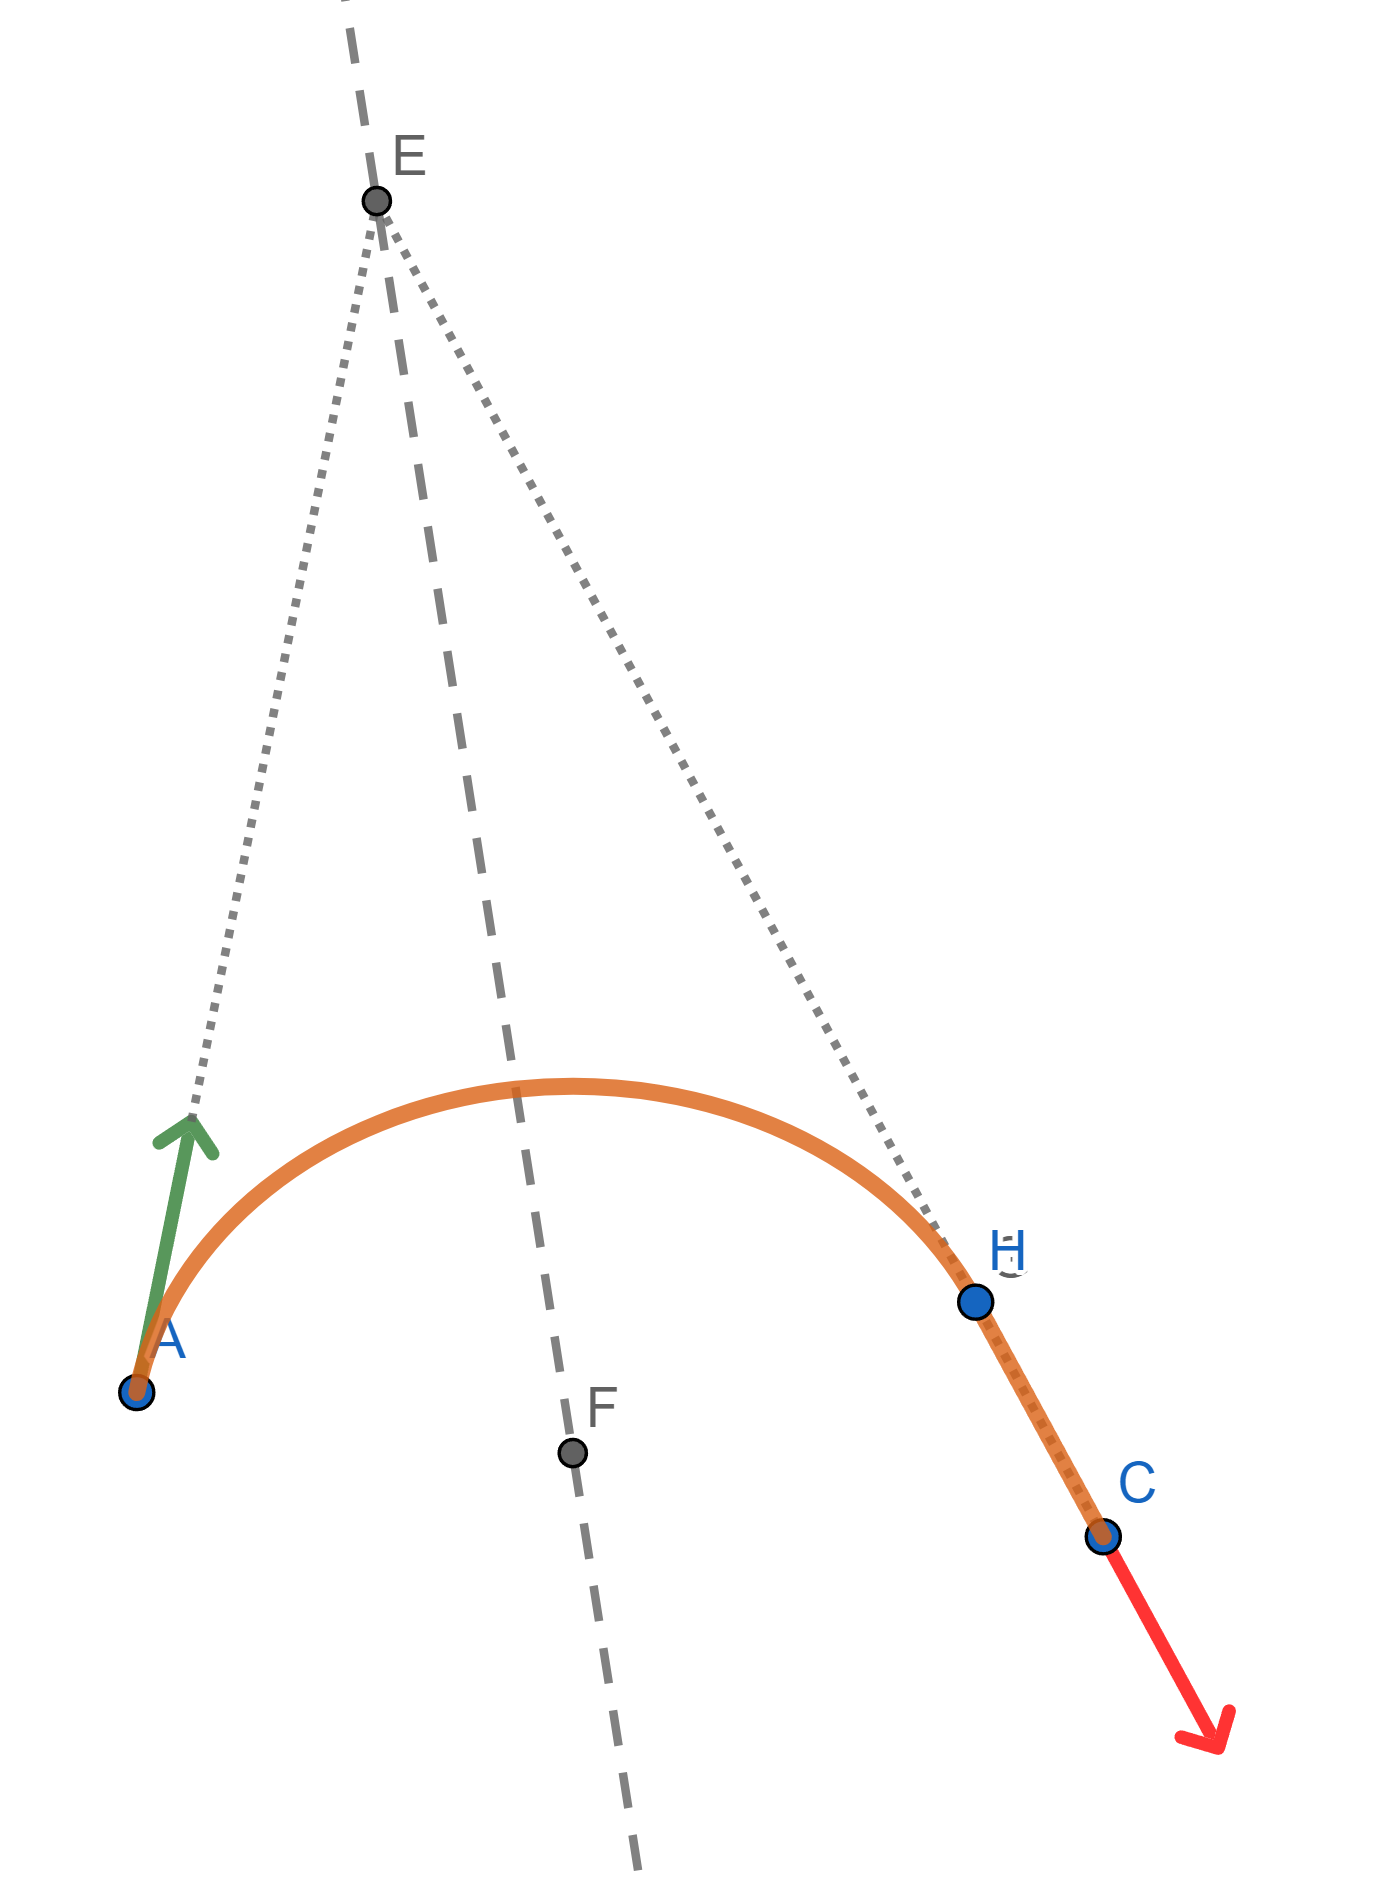
\includegraphics[width=6cm]{screenshots/single-acute-turn-rot-trans.png} & 
    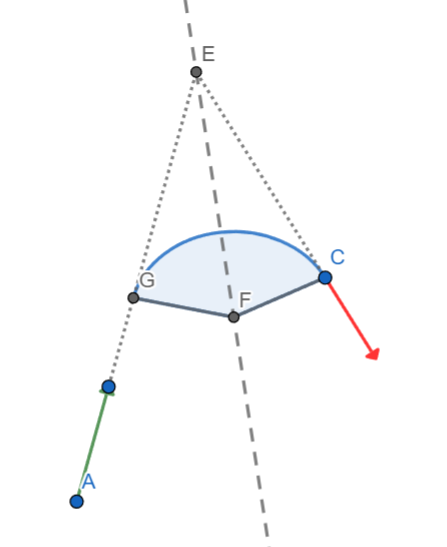
\includegraphics[width=6cm]{screenshots/single-acute-turn-trans-rot.png}       \\
    (a)                                                                      & (b) \\
  \end{tabular}
  \caption{Path planning with a single acute turn}
  \label{fig:path1turnacute}
\end{figure}


\begin{figure}[h]
  \begin{tabular}{cc}
    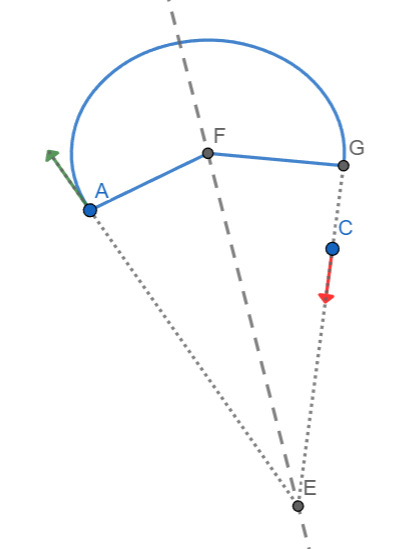
\includegraphics[width=6cm]{screenshots/single-obtuse-turn-rot-trans.png} & 
    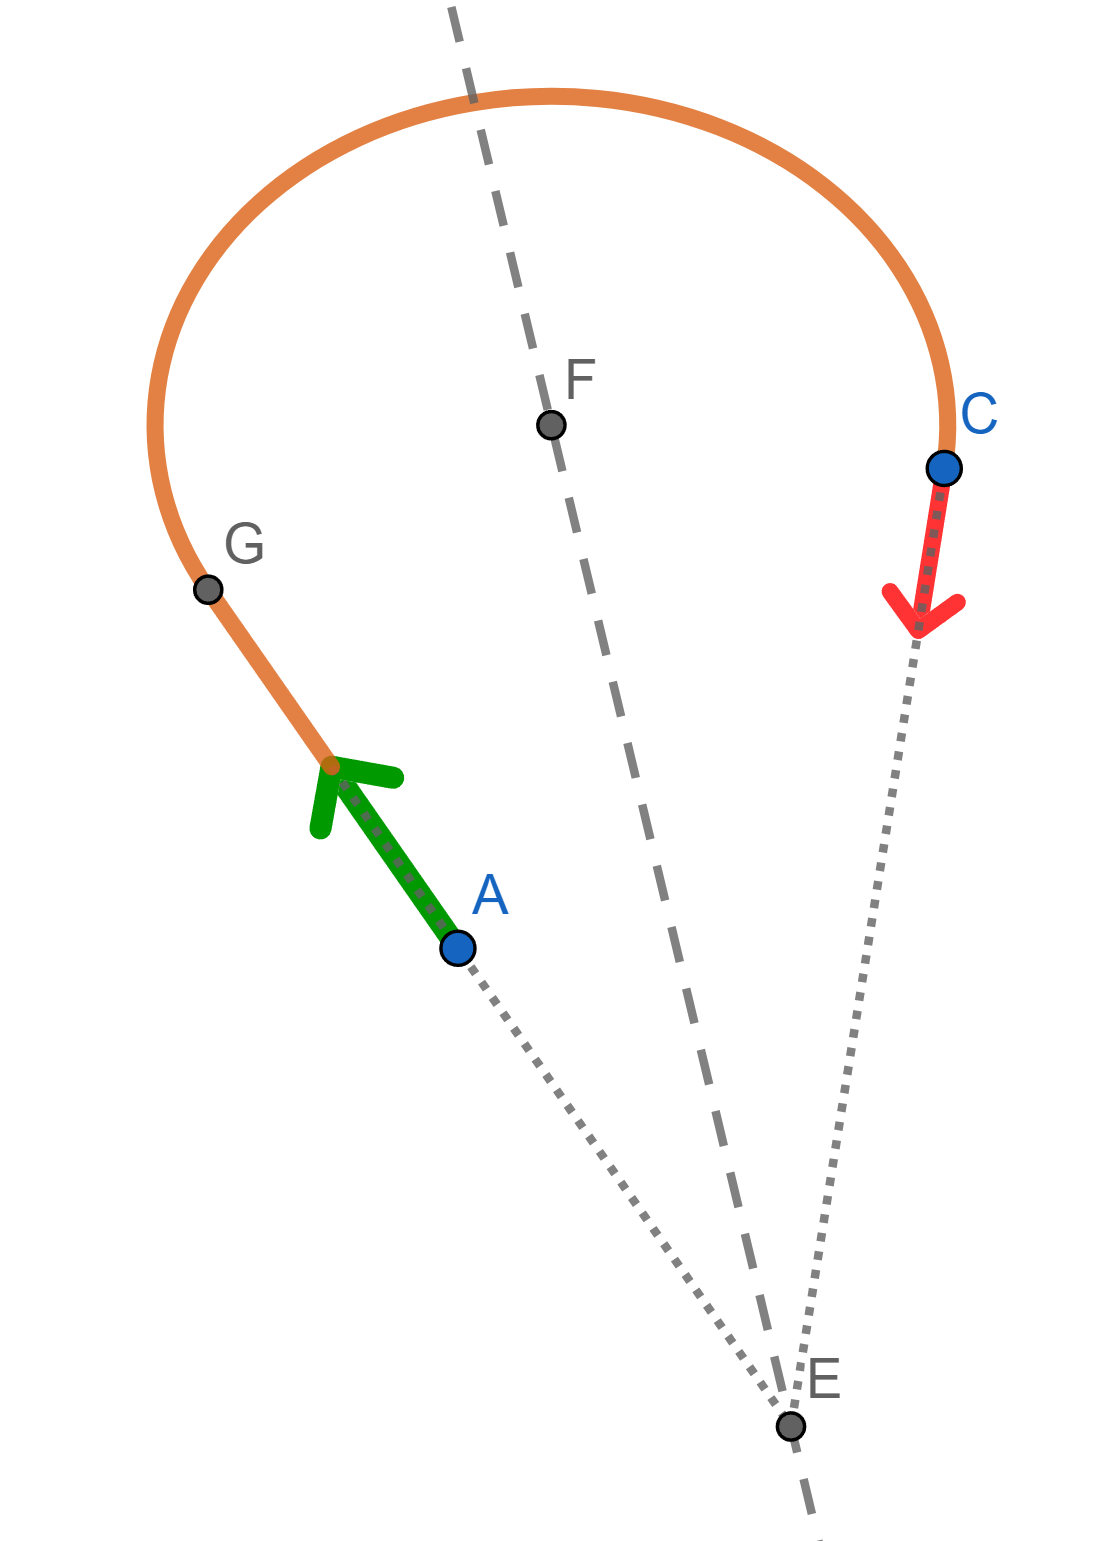
\includegraphics[width=6cm]{screenshots/single-obtuse-turn-trans-rot.png}       \\
    (a)                                                                       & (b) \\
  \end{tabular}
  \caption{Path planning with a single obtuse turn}
  \label{fig:path1turnobtuse}
\end{figure}


There are two cases to consider:
\begin{itemize}
  \item In Figure~\ref{fig:path1turnacute}a, when $|AE| < |CE|$, the bike first rotates from $A$ and $G$ around the
        pivot $F$  before it continues to translate from $G$ to $C$. The pivot of rotation $F$ is the perpendicular
        intersection from $A$ with the angle bisector.
  \item In Figure~\ref{fig:path1turnacute}b, when $|AE| > |CE|$, the bike first translates from $A$ to $G$ before it
        continues to rotate from $G$ to $C$ around the pivot $F$. The pivot of rotation $F$ is determined
        by the perpendicular intersection from $C$ with the angle bisector.
\end{itemize}

In general, when the turn angle is \textbf{acute}, 
i.e. the intersection point is in front of the start $A$ and behind the target $C$, 
the pivot of rotation is determined by the \textbf{closer}
of the starting/target point to the intersection $E$.
However, when the turn angle is \textbf{obtuse}, i.e. the intersection point is in behind the start $A$ and in front of the target $C$, 
the pivot or rotation is determined by the \textbf{further}
point (as shown in Figure~\ref{fig:path1turnobtuse}).

\clearpage
\subsection*{Double Turn Paths}
When the two headings are generally pointing in the same direction, the path can be solved using one translation
and two rotations. The first rotation is an outgoing turn from the start point and the second rotation is
an incoming turn into the target point.
Instead of using one angle bisector, the geometry requires three equal bisectors (as shown by 
the three dashed lines). The second bisector (the center dashed line) defines a placeholder for an intermediate heading 
between the two the turn.

\begin{figure}[hbt]
  \begin{tabular}{cc}
    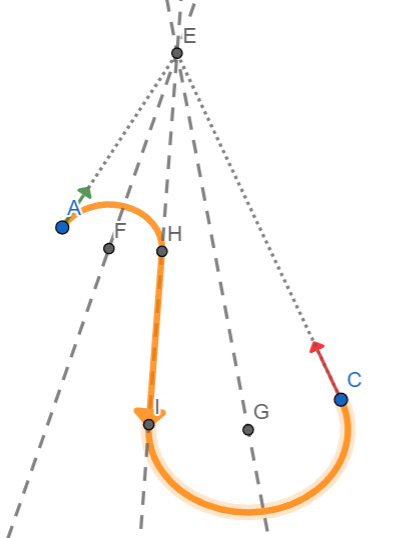
\includegraphics[height=7cm]{screenshots/double-acute-turn-rot-trans.png}
    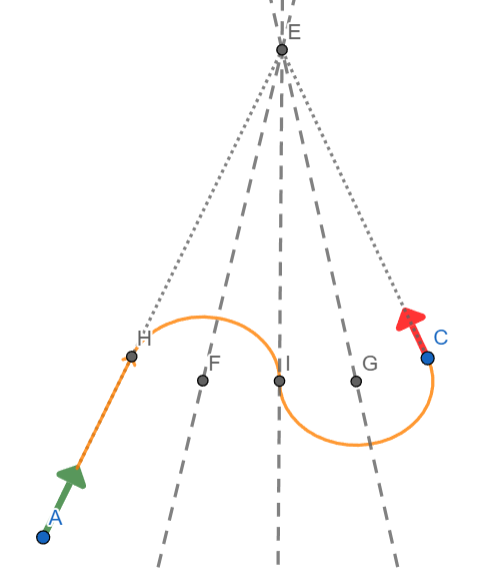
\includegraphics[height=7cm]{screenshots/double-acute-turn-trans-rot.png}
  \end{tabular}
\end{figure}

\begin{itemize}
  \item When start is closer to the intersection $|AE| < |CE|$, the pivot of the
        outgoing turn at $F$ is determined from the perpendicular intersection from $A$
        with the first 3-angle bisector.
  \item When target is closer to the intersection point $|CE| < |AE|$, both
        pivots of rotation ($F$ and $G$, and $|EF| = |EG|$) are determined by the target point.
\end{itemize}

\subsection*{Shorter Double Turn Paths}
The double turn path can be improved two consecutive turning arcs: an outgoing arc from the start point
followed by an incoming arc into the target point. Furthermore, these two arcs can either be 
left-then-right or right-then-left.

In the diagram in Figure~\ref{fig:double-RL} assume the following conditions
\begin{itemize}
  \item Point $P$ is the intersection between the two headings
  \item With respect to the target heading, $P$ is behind the target. Otherwise, the path
        can be solved using a single turn.
  \item The target point $C$ is to the right of the start heading. Otherwise, the solution requires
        a left turn followed by a right turn
  \item Point $M$ is the intersection of the perpendicular of both headings
  \item Point $E$ is the intersection of the target heading and the perpendicular of the start heading
  \item Most importantly, $|EA| < |EC|$ this should allow a right turn which originates from $A$ to ``catch up''
        with the target point $C$
\end{itemize}

\begin{figure}[hbt]
  \begin{tabular}{cc}    
    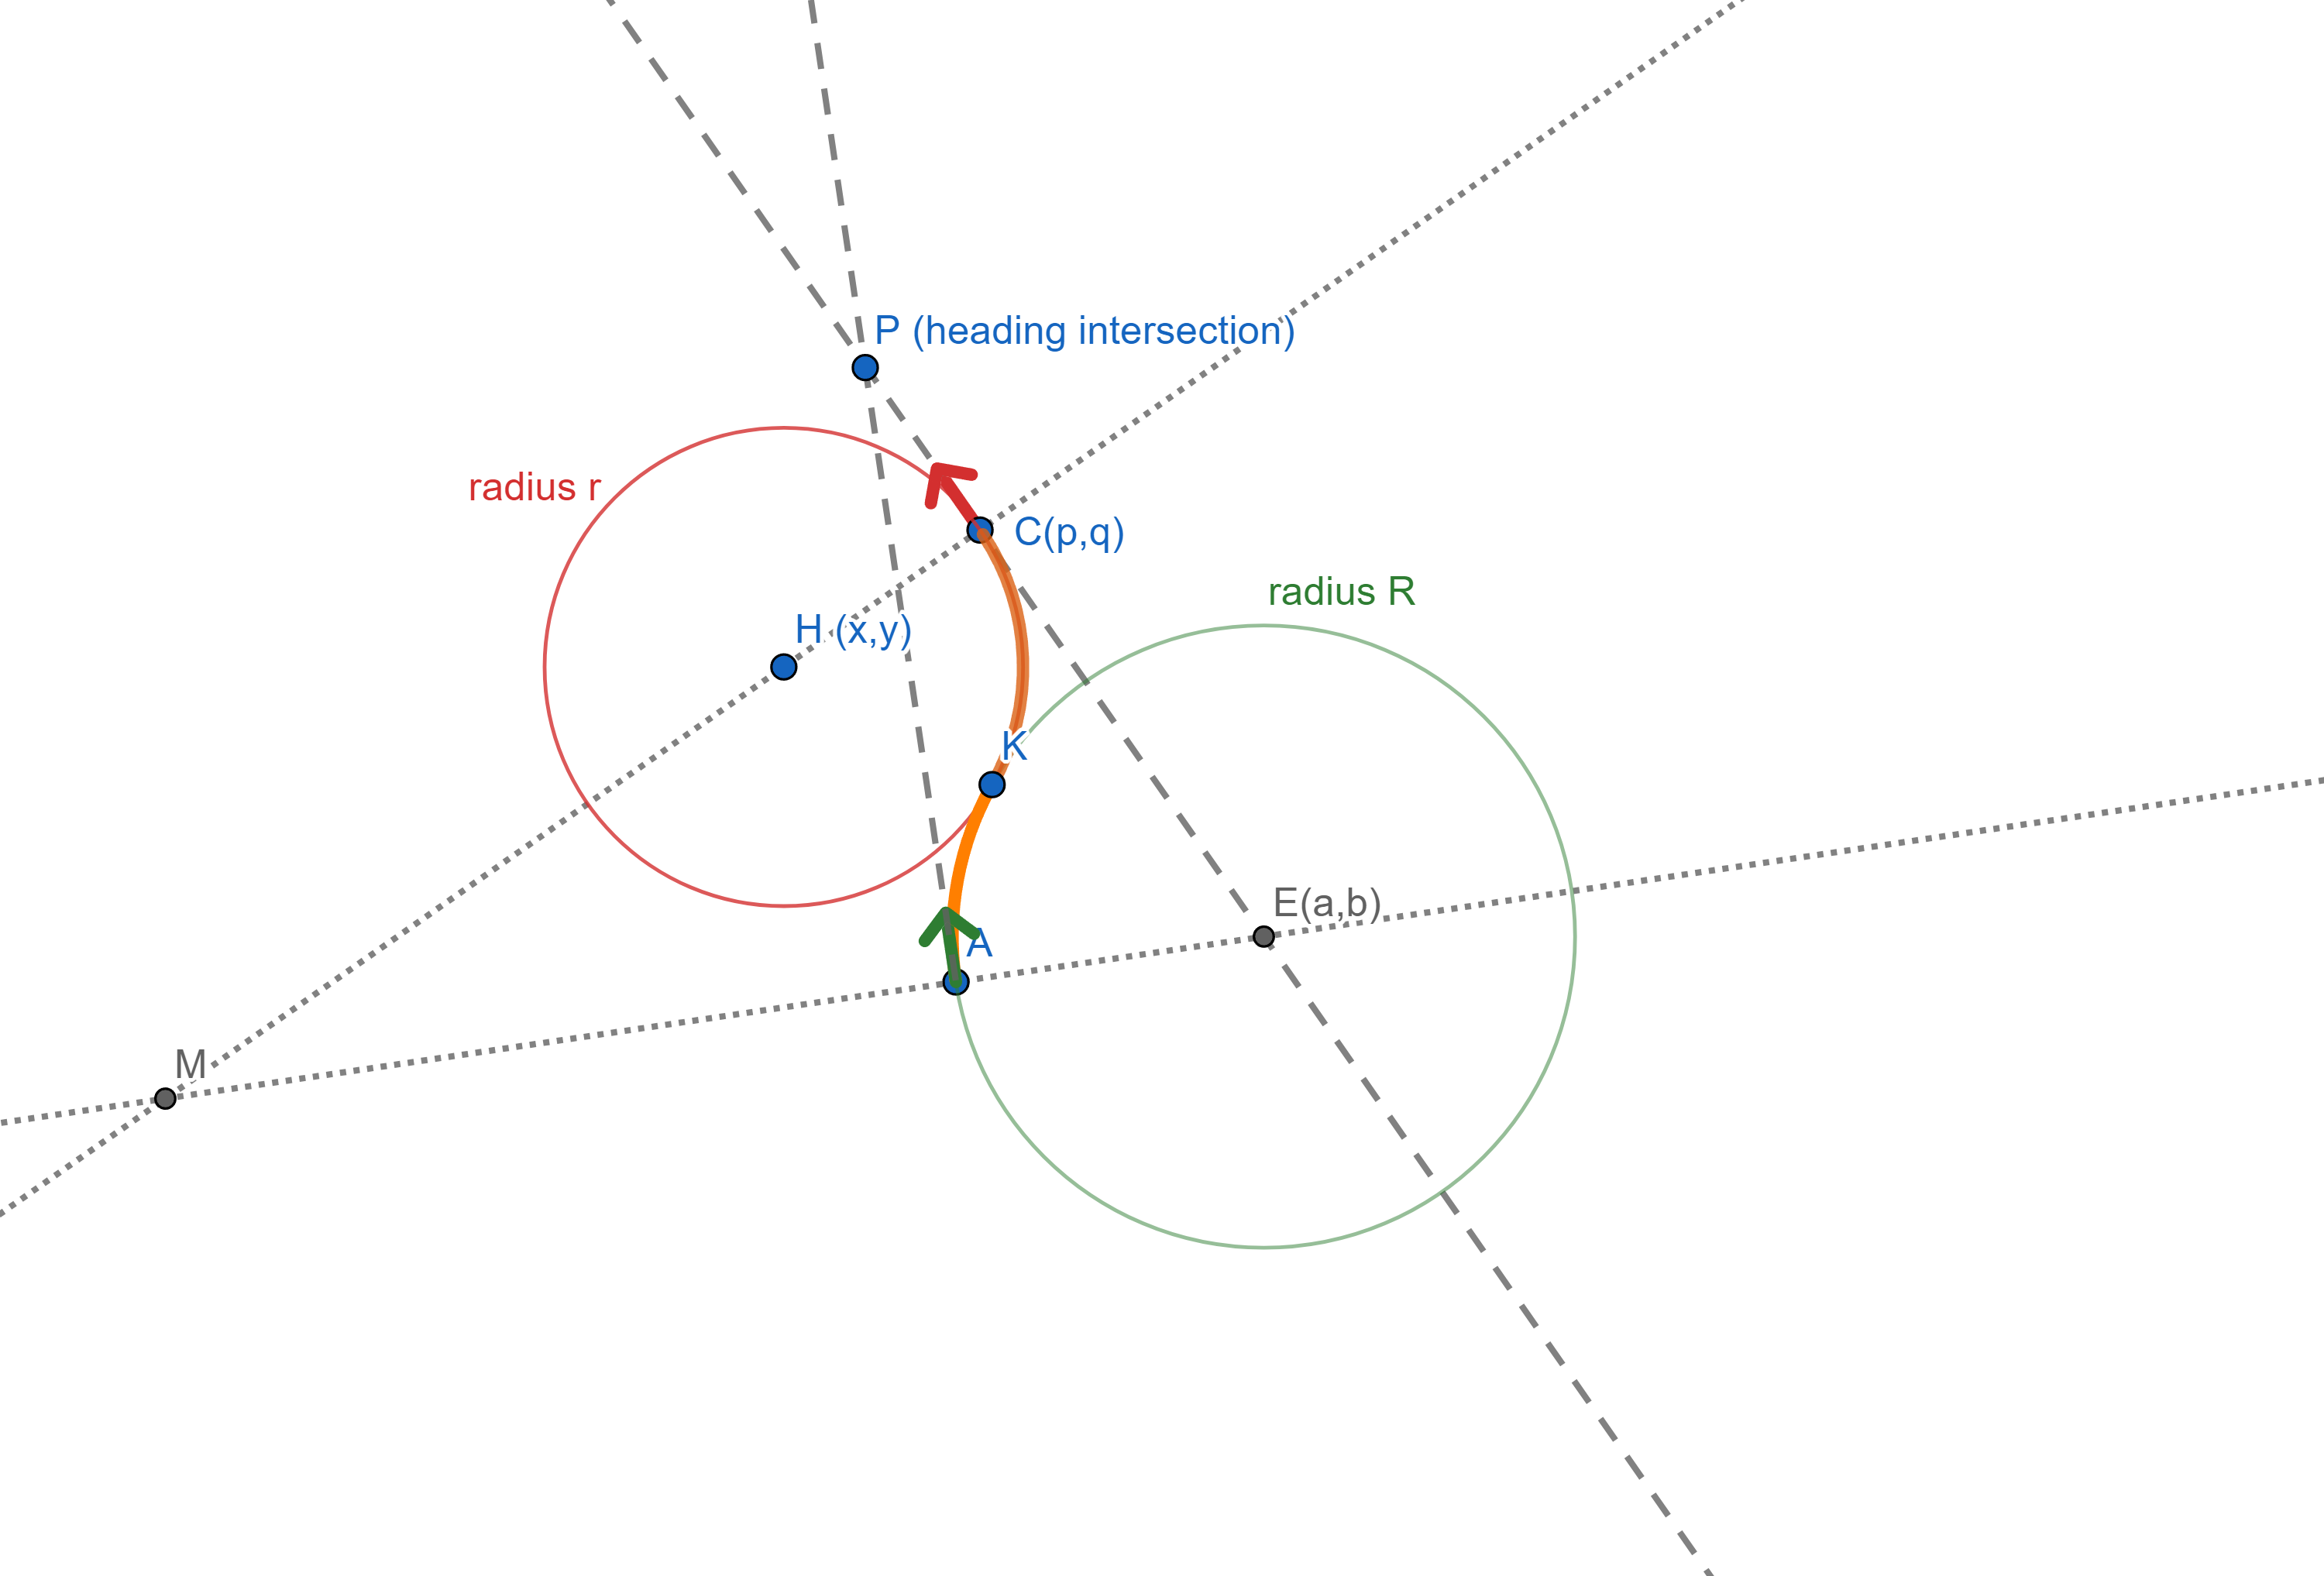
\includegraphics[width=6cm]{screenshots/double-turns-right-left.png} & 
    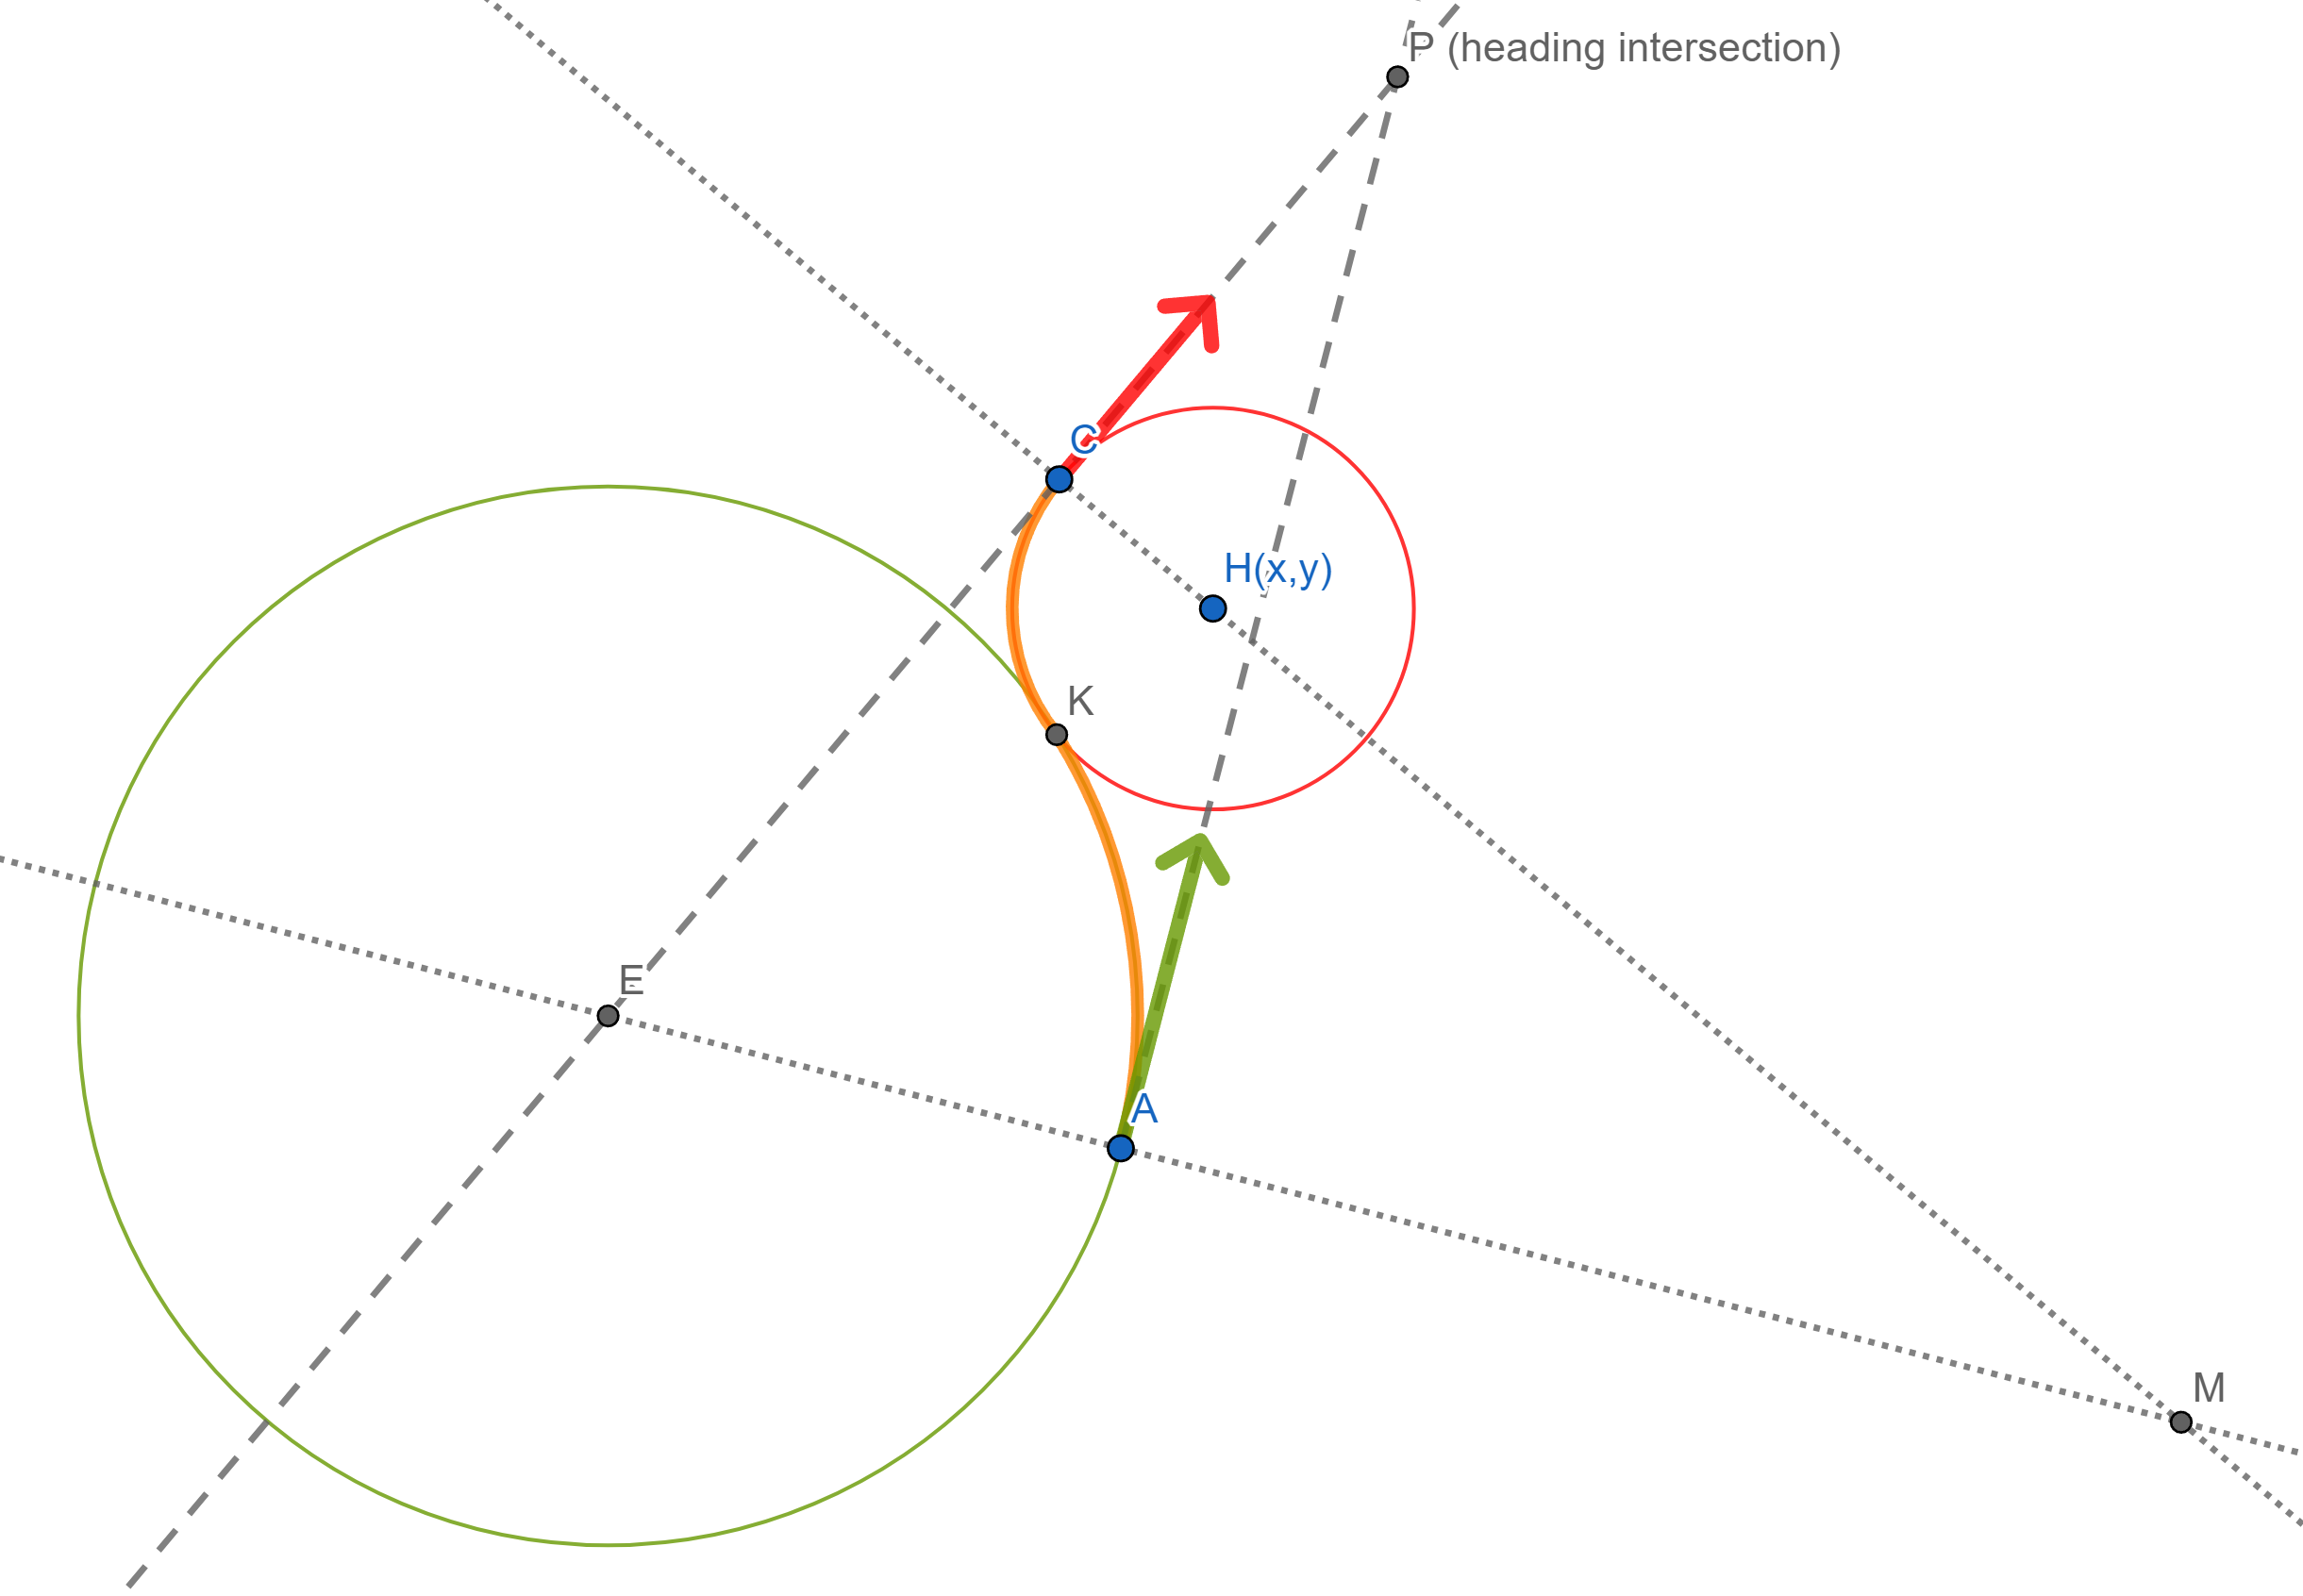
\includegraphics[width=6cm]{screenshots/double-turns-left-right.png}\\
    R-to-L & L-to-R
  \end{tabular}
  \caption{Double Turn Using Consecutive Arcs}
  \label{fig:double-RL}
\end{figure}

The two arcs are determined as followed:

\begin{itemize}
  \item The outgoing arc/circle must be tangent to $A$, and we can select $E$ as its center
  \item The incoming arc must be tangent to $C$ and also tangent to the outgoing circle,
        Hence its center $H$ must be somewhere on $CM$
\end{itemize}
The center $H(x,y)$ must satisfy the following constraints:

\begin{itemize}
  \item $H = \alpha M + (1-alpha) C$
  \item $CH \perp CE$
  \item $|HE| = R + |HK| = R + |CH|$
\end{itemize}

Instead of directly solving the equations analytically, we can apply binary search technique to find $\alpha$
that represents the exact location of $H$ along $CM$.
\end{document}